% !TEX encoding = UTF-8 Unicode
% -*- coding: UTF-8; -*-
% vim: set fenc=utf-8
\documentclass[a4paper,12pt,french]{article}

\usepackage{centrale}
\usepackage{algorithm}
\usepackage{algorithmic}

\hypersetup{
    pdftitle={Parareal Algorithm},
    pdfauthor={Oussama BOUHENNICHE},
    pdfsubject={Parareal Algorithm},
    pdfproducer={Conversion PDF à insérer},
    pdfkeywords={Parareal, euler, Ensemble Kalman Filter, lorenz system} %
}

\DeclareGraphicsRule{.ai}{pdf}{.ai}{.png} % pour insérer des documents .ai
\graphicspath{ {./img/}} % pour ne pas avoir à ajouter eps/ton-image.jpg

% ------------- Packages spéciaux, nécessaires pour ce rapport, à insérer ici ------------- 


\begin{document}

% --------------------------------------------------------------
%                       Page de garde
% --------------------------------------------------------------

\begin{titlepage}
\begin{center}


\includegraphics[width=1\textwidth]{logo.png}\\[1cm]

{\large Master 1 CSMI : Scientific Computation and Mathematics of Innovation}\\[0.5cm]

% Title
\rule{\linewidth}{0.5mm} \\[0.4cm]
{ \huge \bfseries Parareal Algorithm \\[0.4cm] }
\rule{\linewidth}{0.5mm} \\[1.5cm]

% Author and supervisor
\noindent
\begin{minipage}{0.6\textwidth}
  \begin{flushleft} \large
    \emph{Authors :}\\
    Narimane \textsc{ZAOUACHE}
  \end{flushleft}
\end{minipage}%
\begin{minipage}{0.4\textwidth}
  \begin{flushright} \large
    \emph{Supervisors :} \\
    M.~Christophe \textsc{Prud'homme}
  \end{flushright}
\end{minipage}

\vfill

% Bottom of the page
{\today}

\end{center}
\end{titlepage}

% --------------------------------------------------------------
%                            Abstract
% --------------------------------------------------------------
\newpage
\thispagestyle{empty}

\vspace*{\fill}
\noindent\rule[2pt]{\textwidth}{0.5pt}\\
{\textbf{Abstract :}}
This study explores the application of the Ensemble Kalman Filter (EnKF) to nonlinear dynamic systems, 
specifically the Lorenz system, and analyzes its effectiveness based on various experimental parameters. 
By utilizing an experimental setup based on numerical resolutions of the Lorenz system, 
we implemented the EnKF and evaluated its performance by testing the filter with simpler systems,
 such as ordinary differential equations (ODEs). 
 The impact of the observation covariance matrix $R$ and the number of ensembles was also analyzed.
  The results demonstrate how these factors influence the filter's accuracy and uncertainty, 
  as well as the effect of noisy observations on the quality of the predictions.

{\noindent\textbf{keywords :}}
Ensemble Kalman Filter (EnKF), Explicit Euler, , Lorenz system
\\
\noindent\rule[2pt]{\textwidth}{0.5pt}

\vspace*{\fill}
\newpage

% --------------------------------------------------------------
%                    Table des matières 
% --------------------------------------------------------------

\thispagestyle{empty}
\tableofcontents
%\newpage

% --------------------------------------------------------------
%                         Début du corps
% --------------------------------------------------------------
\newpage
\section{Introduction}
The Lorenz system, known for its chaotic properties, 
is often used as a testbed for filtering and forecasting techniques. 
The Ensemble Kalman Filter (EnKF) is a popular method for nonlinear systems.
 This report describes the application of the EnKF to the Lorenz system, 
 using numerical methods to solve the differential equations 
 and analyze the performance of the EnKF in terms of accuracy and uncertainty.


% --------------------------------------------------------------
%                         Partie 1
% --------------------------------------------------------------

\newpage
\section{Background}
\subsection{Lorenz system:}

The Lorenz system \cite{lorenz} is a mathematical model that illustrates how dynamic systems can exhibit chaotic behavior.
 It was introduced by Edward Lorenz in 1963,
  primarily to model atmospheric convection.

The Lorenz system is a set of three coupled, 
nonlinear differential equations:

\begin{equation}
    \begin{cases}
        \displaystyle\frac{dx}{dt} = \sigma(y - x) \\
        \displaystyle\frac{dy}{dt} = x(\rho - z) - y \\
        \displaystyle\frac{dz}{dt} = xy - \beta z
    \end{cases}
\end{equation}

where:
\begin{itemize}
    \item $x$, $y$ and $z$ represent the system state,
    \item $\sigma$, $\rho$ and $\beta$ are parameters that influence the system's behavior.
\end{itemize}

These equations model thermal convection in a fluid layer and are known 
to generate chaotic behavior under certain parameter conditions.

\subsection{The Ensemble Kalman Filter}
The Ensemble Kalman Filter (EnKF) was developed by Geoffrey Evensen \cite{iglesias2013ensemble}. 
The concept was introduced in a 1994 paper titled "Sequential Data Assimilation with a Nonlinear Quasi-Geostrophic Model Using the Ensemble Kalman Filter.

The EnKF is a state estimation method for nonlinear and stochastic systems, as well as high-dimensional problems.

The fundamental principle of the EnKF is based on propagating an ensemble of state samples through a dynamic model and updating these samples based on observations.

\textbf{Propagation through the Model :}
Each member of the ensemble is independently propagated through the dynamic model to obtain a forecast of the future state.

\textbf{Update with Observations :}
The forecasts are then adjusted based on the available observations to produce an updated state estimate \cite{wikipediaEnKF}.

\subsubsection{EnKF Algorithm Steps} 
\textbf{1. Initialization}
   Generate an initial set of state samples $\{x_i^0 \}_{i=1}^N$, where $N$ is the number of samples. These samples are randomly drawn according to an assumed initial state distribution. Typically, they are generated by perturbing an initial estimate $x_0$ with a noise distribution, modeled by a multivariate normal distribution with a mean $x_0$ and an initial covariance matrix $P$.\\
\textbf{2. Prediction Step:}
   For each member of the ensemble, propagate the state through the model to obtain the predicted state:

   $$x_i^{\text{pred}} = f(x_i^{\text{upd}}) + w_i$$

   where:
   \begin{itemize}
    \item ${x}_i^{\text{upd}}$ est l'état d'analyse du membre $i$ à partir de l'étape précédente.
    \item $f(x)$ est la fonction de transition d'état qui décrit la dynamique du système.
    \item $w_i$ est un vecteur de bruit de processus tiré aléatoirement, représentant les incertitudes du modèle, souvent modélisé comme une variable aléatoire gaussienne avec une moyenne nulle et une matrice de covariance $Q$.
   \end{itemize}
\textbf{3. Update Step}  
   The available observations are used to correct the forecasts and adjust the state samples. For each member of the ensemble, a simulated observation $z_i^{\text{pred}}$ is calculated using:
   $$z_i^{\text{pred}} = h(x_i^{\text{pred}}) + v_i$$
   where:
   \begin{itemize}
    \item $h(x)$ is the observation function that relates the state to the measurements,
    \item $v_i$  is a measurement noise vector drawn randomly, often modeled as a Gaussian random variable with zero mean and covariance matrix $R$.
   \end{itemize}


   The forecasts are updated by calculating the Kalman gain, which is used to adjust the forecasts based on the observations:
   $$K_k = P_k^{\text{pred}} H^T (H P_k^{\text{pred}} H^T + R)^{-1}$$

   where $H$ is the Jacobian matrix of the observation function. The Kalman gain $K_k$ is then used to adjust the predicted states:
   $$ x_i^{\text{upd}} = x_i^{\text{pred}} + K_k (z_k - h(x_i^{\text{pred}}) + v_i)$$

   where $z_k$ is the observed measurement at time $k$.
\subsection{Explicit Euler}

The explicit Euler method is a simple and commonly used technique for solving ordinary differential equations (ODEs). It approximates the solution of an ODE by advancing in small increments from a known initial condition.

Consider a first-order ODE of the form:

$$
\frac{dy}{dt} = f(t, y), \quad y(t_0) = y_0,
$$

The explicit Euler method uses the following iterative formula to advance the solution from $t_n$ to $t_{n+1}$:

$$
y_{n+1} = y_n + h \cdot f(t_n, y_n).
$$ 



% --------------------------------------------------------------
%                            Partie 2
% --------------------------------------------------------------

\section{Methodology}
\subsection{Host Organization}

\subsubsection{Overview}
 The study was conducted in collaboration with the Cemosis 
 laboratory \cite{cemosis}, which specializes in scientific computing,
 mathematical modeling, and industrial applications. 
 Cemosis works closely with academic institutions and 
 industrial partners to develop innovative solutions in
 computational science and engineering. The goal of this 
 project is to test and evaluate the effectiveness of the
 Ensemble Kalman Filter (EnKF) applied to the chaotic
 Lorenz system, which is known for its unpredictable behavior.

\subsubsection{Use of the Filterpy Library}
Filterpy \cite{filterpy} was one of the main tools used in this study. 
This library, widely recognized for its efficient 
implementations of various Kalman filters, provided the 
necessary tools to robustly and flexibly implement the 
Ensemble Kalman Filter (EnKF).

It facilitated the implementation of the EnKF by offering 
predefined classes and functions for ensemble management, 
state propagation, and observation-based updates. 
Additionally, it allowed for easy customization of filter 
parameters, such as ensemble size, covariance matrix, 
and state transition functions.

The use of Filterpy was therefore crucial for the efficiency 
and accuracy of the simulations carried out in this study.

\subsection{Experimental Setup}
\subsubsection{Numerical Solution of the Lorenz System}
The Lorenz system, modeled by a set of nonlinear differential 
equations, was solved numerically using the explicit Euler 
method. This method was chosen for its simplicity and 
effectiveness in the context of a dynamic system where 
small time steps are necessary to capture the details of 
chaotic behavior.

The equations of the Lorenz system, with standard parameters 
$\sigma = 10$, $\rho = 28$, and $\beta = \frac{8}{3}$, 
were solved over the time interval [0, 20] with an initial 
condition $u_0= (5., -5., 20.)$.
\subsubsection{Implementation of the EnKF}

The EnKF was used to estimate the state of the Lorenz 
system by integrating noisy synthetic observations. 
These observations, generated from the system's true state 
with added noise, were used to update the state estimates 
at each time step.


\paragraph{Steps of the EnKF on the Lorenz System}
\vspace{0.5cm} 

\begin{itemize}
  \item \textbf{1. Ensemble Initialization:} The state ensembles were initialized around the known initial condition $u_0 = 5., -5., 20.$, with a random perturbation to introduce initial uncertainty.
  \item \textbf{2. State Propagation:} Each state vector was propagated independently through the dynamics of the Lorenz system using the explicit Euler method.
  \item \textbf{3. Update with Observations:} At each time step, synthetic observations were used to correct the EnKF predictions by adjusting the estimated states based on the difference between the predictions and the observations.
\end{itemize}

After applying the EnKF, the estimated trajectories were 
compared to the actual trajectories of the Lorenz system to 
verify the accuracy of the filter. This comparison revealed 
the discrepancies between the estimated and actual trajectories, 
allowing for the calculation of absolute errors, 
a key measure of EnKF performance. 
The uncertainty of the estimates was also assessed 
by observing the spread of the ensembles around the true 
states, which helped to explain the deviations observed in the 3D plots.

\subsubsection{Tests with Simpler Systems (ODEs)}
Before applying the Ensemble Kalman Filter (EnKF) to the 
Lorenz system, preliminary tests were conducted on simpler 
ordinary differential equations (ODEs) to validate the EnKF implementation. These simpler ODEs serve as a testbed to understand the behavior of the filter in less complex contexts.
\begin{itemize}
  \item    \textbf{Test 1 :} Solving the ODE   $\frac{dy}{dt} = -t \cdot y^2$.

The equation is solved with the initial condition  
$y(0)=1.0$ using the explicit Euler method. The time step 
used is  $dt=0.05$ for a total duration ofde $T=4.0$.
The EnKF is configured with an ensemble of $N=20$ members, 
generating initial perturbations around $y_0=1.0$ 
to simulate uncertainties. The state transition function 
is defined as $f(x, dt) = x - t \cdot x^2 \cdot dt $, while the observation function is $h(x)=x$. The process and observation 
covariances are set to $Q=0.01$ and $R=0.1$, respectively.


\item     \textbf{Test 2:} Solving the ODE $\frac{dy}{dt} = -y + cos(t)$.

The equation is solved starting with the initial condition 
$y(0)=0.0$  using the explicit Euler method. The time step 
is $dt=0.05$, and the simulation runs for a total duration 
of $T=5.0$. The EnKF is configured with an ensemble of 
$N=20$ members, with initial perturbations around $y_0=0.0$ 
to simulate uncertainties. The state transition function 
is defined as $f(x, dt) = x - x \cdot dt + \cos(t) \cdot dt $, and the 
observation function is $h(x)=x$. The process and 
observation covariances are set to $Q=0.01$ and $R=0.1$, respectively.
\end{itemize}

\subsubsection{Impact of the Observation Covariance Matrix $R$}
The observation covariance matrix $R$ plays a crucial role in the performance 
of the EnKF by directly influencing the accuracy of trajectory estimates. 
$R$ represents the confidence assigned to the observations; a lower value 
of $R$ indicates observations that are considered more reliable, 
while a higher value indicates more noisy observations.

In this study, we analyzed the impact of different values of $R$ (0.1, 1.0, and 5.0) 
on trajectory estimates. The goal is to determine how the confidence given 
to the observations affects the EnKF's ability to correct its predictions 
and track the underlying system.

\subsubsection{Impact of the Number of Ensembles $N$}

A series of experiments was conducted to evaluate the 
impact of the number of ensembles $N$ on the performance 
of the EnKF. For each value of $N$ (10, 20, 50, 100), 
the estimated trajectories were compared to the actual 
trajectories of the Lorenz system. The absolute errors 
and uncertainties associated with the estimates were 
analyzed to understand how the number of ensembles affects 
the performance of the EnKF.

\subsubsection{Visualization of Results}
The results of the experiment were visualized by plotting 
the real and estimated trajectories in the phase space 
$(x, y, z)$. Absolute error graphs as a function of time 
were also produced for each configuration of $N$ and $R$, 
highlighting the effectiveness of the EnKF and the influence 
of the number of ensembles on the accuracy of the predictions.

\section{Results and Analysis}
\subsection{EnKF Trajectories and Deviations}

The results show that the trajectory estimated by the EnKF (orange curve) generally follows the true trajectory, but with some deviations. These deviations are particularly noticeable when the observations are noisy, impacting the accuracy of the filter's updates.
\begin{figure}[H]
  \centering
  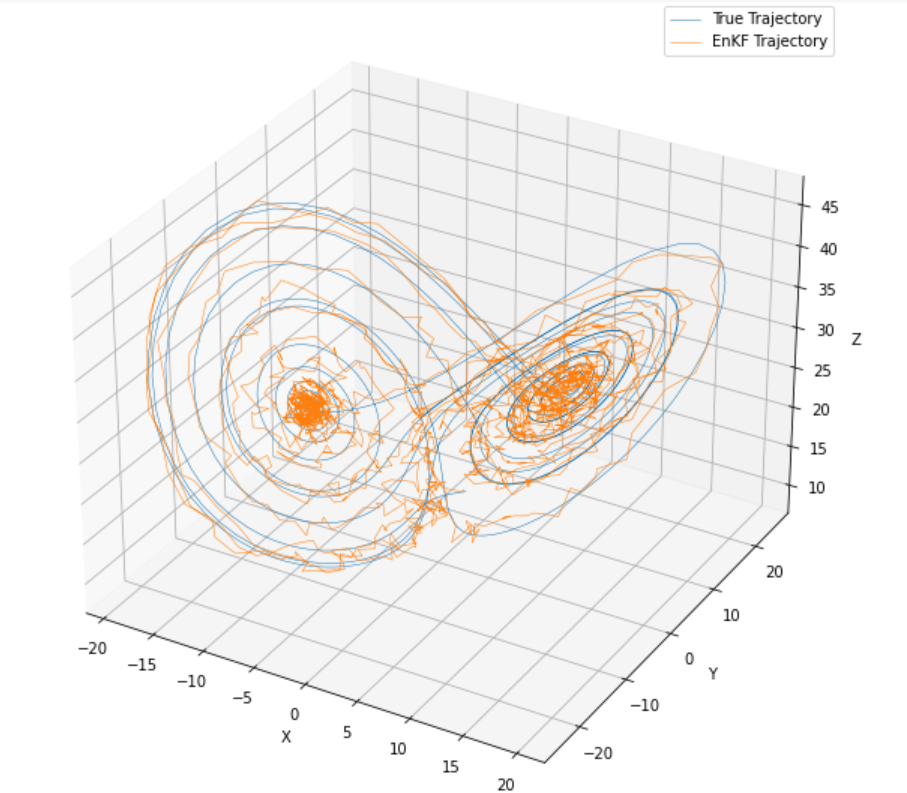
\includegraphics[width=0.45\textwidth]{img/lorenz_enkf.png}
  \caption{Lorenz System Solved by Euler explicit Method with Ensemble Kalman Filter}
  \label{fig:6}
\end{figure}
\newpage

\subsection{Uncertainty of Estimates}
The graphs show a relatively low uncertainty, around 0.75, for all three dimensions $(X, Y, Z)$. This indicates that the Ensemble Kalman Filter maintains good confidence in its predictions, despite the chaotic behavior of the Lorenz system.

\begin{figure}[H]
  \centering
  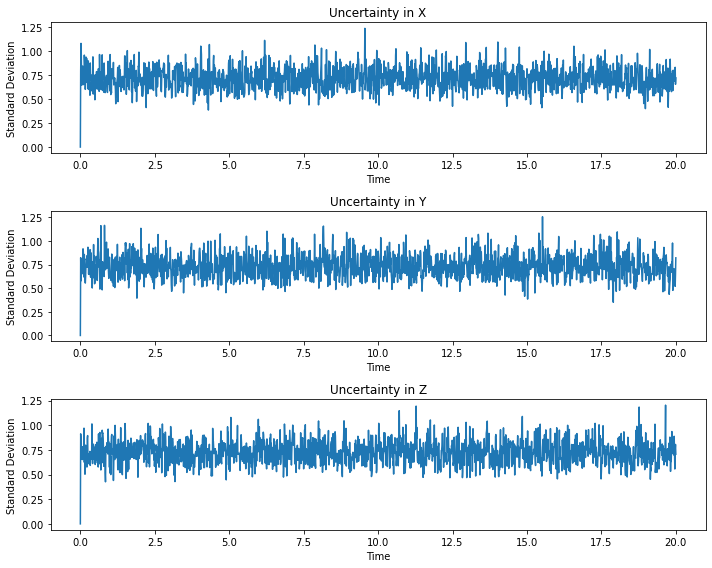
\includegraphics[width=0.7\textwidth]{img/incertitude.png}
  \caption{Uncertainty}
  \label{fig:6}
\end{figure}



\subsection{Individual Trajectories and Absolute Errors}
The graphs of individual trajectories show that the Ensemble Kalman Filter (EnKF) accurately follows the dynamics of the Lorenz system, although some divergences do appear. The absolute errors generally remain below 2, with a few peaks reaching up to 2.5. These errors indicate the moments when the EnKF struggles to follow the true trajectory.

\begin{figure}[H]
  \centering
  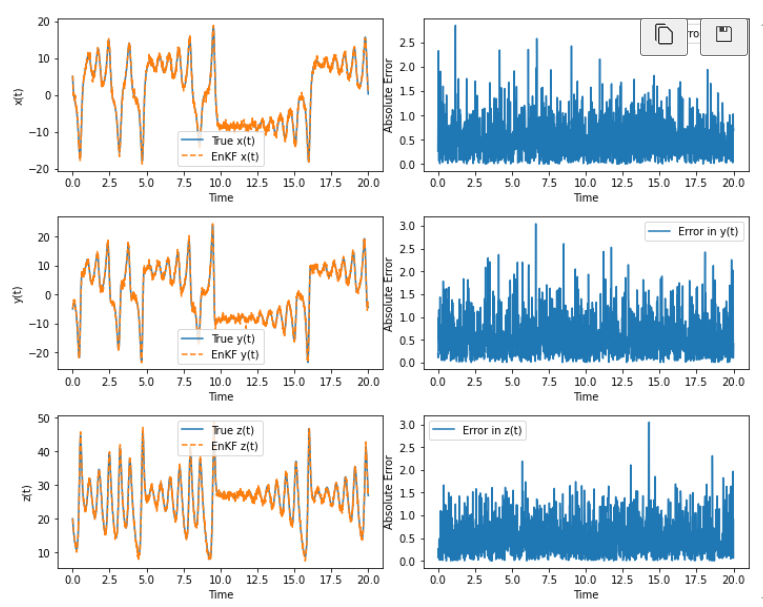
\includegraphics[width=0.7\textwidth]{img/erreur_abs.png}
  \caption{Individual Trajectories and Absolute Errors}
  \label{fig:6}
\end{figure}




\subsection{Impact of Noisy Observations}
The results reveal that increasing $R$ (indicating noisier observations) has a significant impact on the quality of the EnKF estimates. With higher values of $R$, the EnKF struggles to properly adjust its predictions to the observations, resulting in increased divergence between the estimated trajectory and the true trajectory. The growing uncertainty observed for $R=5.0$ reflects this difficulty in reliably correcting predictions, making the estimates more prone to errors.

\begin{figure}[ht!]
  \centering
  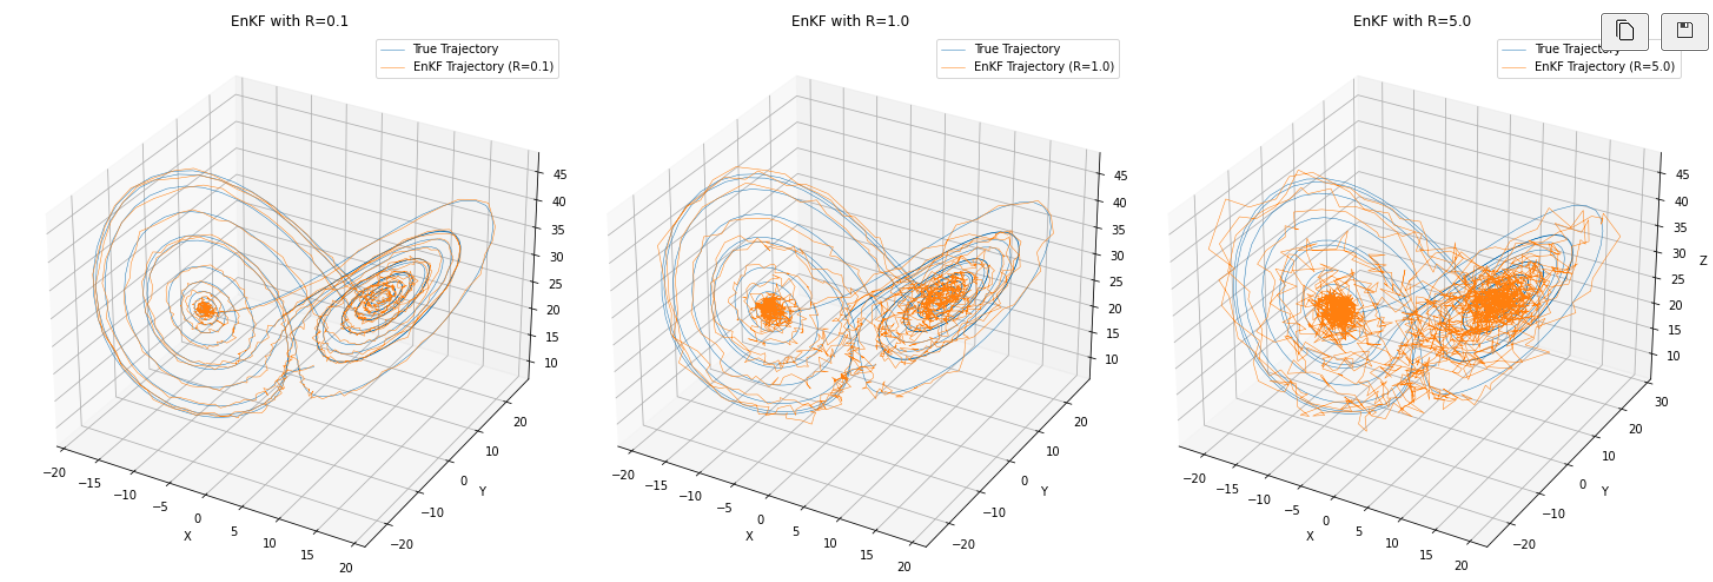
\includegraphics[width=0.7\textwidth]{img/Matrice_d_observation.png}
  \caption{Lorenz System Solved by Euler explicit Method with Ensemble Kalman Filter with different values of $R$}
  \label{fig:6}
\end{figure}
\newpage

\subsection{Influence of the Number of Ensembles ($N$)}

By varying the number of ensembles $N$, we observe that even with $N=10$, the estimated trajectory closely follows the true trajectory, though with less detail. With $N=20$ and $N=50$, the precision improves, and with $N=100$, the trajectory becomes slightly smoother and better matches the true trajectory. The uncertainty also decreases as $N$ increases, indicating greater confidence in the estimates.

\begin{figure}[ht!]
  \centering
  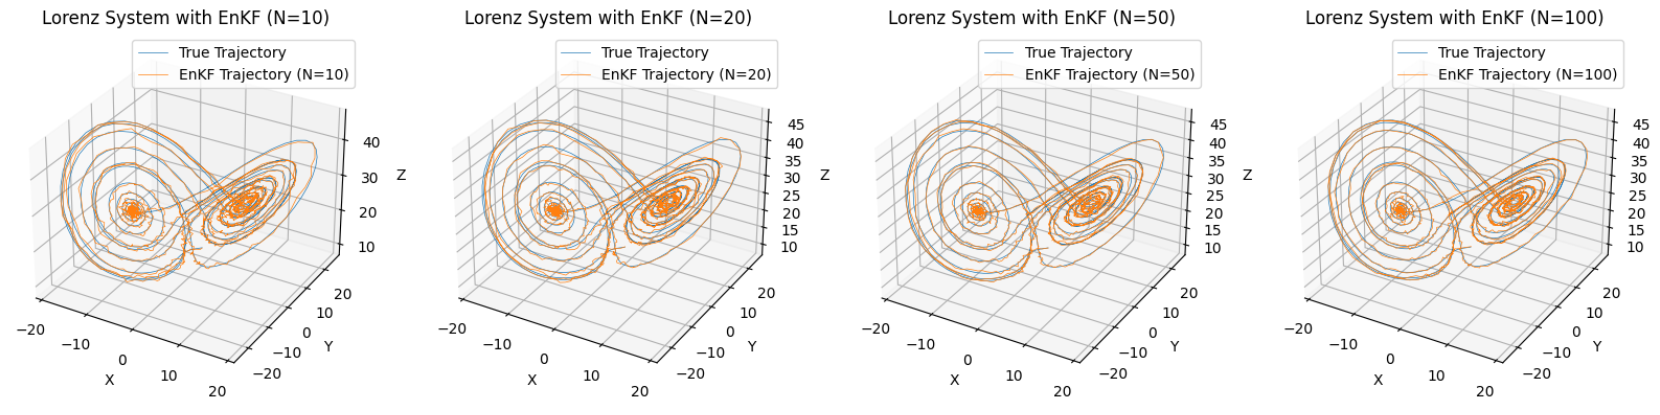
\includegraphics[width=0.7\textwidth]{img/ensemble_N.png}
  \caption{Lorenz System Solved by Euler explicit Method with Ensemble Kalman Filter with different values of $N$}
  \label{fig:6}
\end{figure}



\section{Discussion}
\subsection{Accuracy and Reliability of the EnKF}
The results demonstrate the Ensemble Kalman Filter's (EnKF) ability to track the complex and chaotic dynamics of the Lorenz system, even in the presence of significant uncertainties. By incorporating noisy observations, the filter continuously adjusts its predictions to align with the actual trajectory of the system. These adjustments are observable as small oscillations around the true trajectory, reflecting the corrections made by the EnKF at each observation step.

However, the chaotic nature of the Lorenz system means that small errors, initially minimal, gradually accumulate and result in noticeable deviations in the estimated trajectories compared to the true trajectory. Despite these challenges, the observed uncertainties remain relatively low, indicating that the dispersion of the ensembles around the mean is moderate. This suggests that the EnKF maintains a good level of confidence in its predictions, despite the inherent fluctuations of the system.

Indeed, while the Lorenz system tends to amplify errors due to its chaotic behavior, the EnKF manages to keep these errors within a relatively narrow range, ensuring that the estimates remain close to the true values. This performance reflects the effectiveness of the Ensemble Kalman Filter in modeling and predicting complex systems, while managing the uncertainties associated with noisy observations.
\subsection{Impact of the Observation Matrix}
The impact of the observation covariance matrix $R$ is crucial for the performance of the EnKF filter. A low value of $R$ (e.g., 0.1) makes the filter more sensitive to observations, giving them excessive trust, even if they are noisy. This leads the filter to strongly correct the model's estimates, closely following the system's true trajectory. However, this approach can introduce small oscillations due to observational noise. Despite this, the filter effectively minimizes errors and uncertainties, keeping the trajectory close to the actual system behavior.

In contrast, a high $R$ value (e.g., 5.0) makes the filter more conservative, giving less weight to observations and relying more on the model. The filter then applies fewer corrections, favoring model predictions that it deems more reliable than noisy observations. While this approach can be useful when observations are uncertain, it may fail to capture the full complexity of the system's dynamics, leading to increased errors, greater divergence from the true trajectory, and growing instability.

In summary, a compromise is needed:
$R$ must be low enough for the filter to effectively utilize observations, but high enough to avoid overconfidence in noisy data. Therefore, careful calibration of $R$ is essential to balance the trust placed in observations and the model, ensuring accurate and reliable state estimates.

\subsection{Importance of the Number of Ensembles}
The Lorenz system is known for its chaotic behavior, where small differences in initial conditions can lead to significant divergences in the system's trajectories over time.

When the number of ensembles $N$ is low, the Ensemble Kalman Filter (EnKF) fails to fully capture the complexity and variability of the chaotic system. Each ensemble represents an estimate of the system's state, but with few ensembles, these estimates only cover a limited portion of the possible state space. This results in insufficient coverage of the different trajectories the system might follow. Consequently, the estimates can be coarse, inadequately reflecting the diversity of possible system behaviors, and leading to an underestimation of the true uncertainty. This situation can cause biases in forecasts and reduce their accuracy.

In contrast, a higher number of ensembles $N$ significantly improves the performance of the EnKF. With a larger $N$, the ensemble of estimates covers a broader range of possibilities for the system's state, meaning that the diversity of potential trajectories is better captured. This more comprehensive coverage of the state space allows for better representation of possible variations and inherent uncertainties. As a result, state updates based on observations become more accurate, and prediction errors are reduced. Additionally, a larger $N$ helps to mitigate statistical noise caused by random fluctuations by providing a more stable estimate that is less sensitive to random variations. This leads to more reliable and robust results. However, it is important to note that increasing the number of ensembles comes with computational costs. Therefore, it is essential to find a balance between the number of ensembles and the available resources to achieve optimal results.

\subsection{Limitations and Perspectives}

Despite its effectiveness, the Ensemble Kalman Filter (EnKF) has certain limitations, particularly in managing chaotic systems and very noisy conditions. One of the main limitations is related to the filter's sensitivity to initialization errors and model parameters, which can affect the accuracy of estimates, especially in highly nonlinear systems like the Lorenz system. Additionally, the choice of the number of ensembles $N$ and the observation covariance matrix $R$ can significantly impact the filter's performance, requiring careful calibration to avoid underestimation or overconfidence in the observations. In the future, it would be relevant to explore techniques to improve ensemble initialization, optimize filter parameters, and develop methods to better handle extreme uncertainties and nonlinearities in order to enhance the robustness and accuracy of the filter under various conditions.



   

%\subsubsection*{Implementation}
%
%We implement the adaptive RK4 (see \reff{fig:4}) method in python.
%
%\begin{figure}[ht!]
%    \centering
%    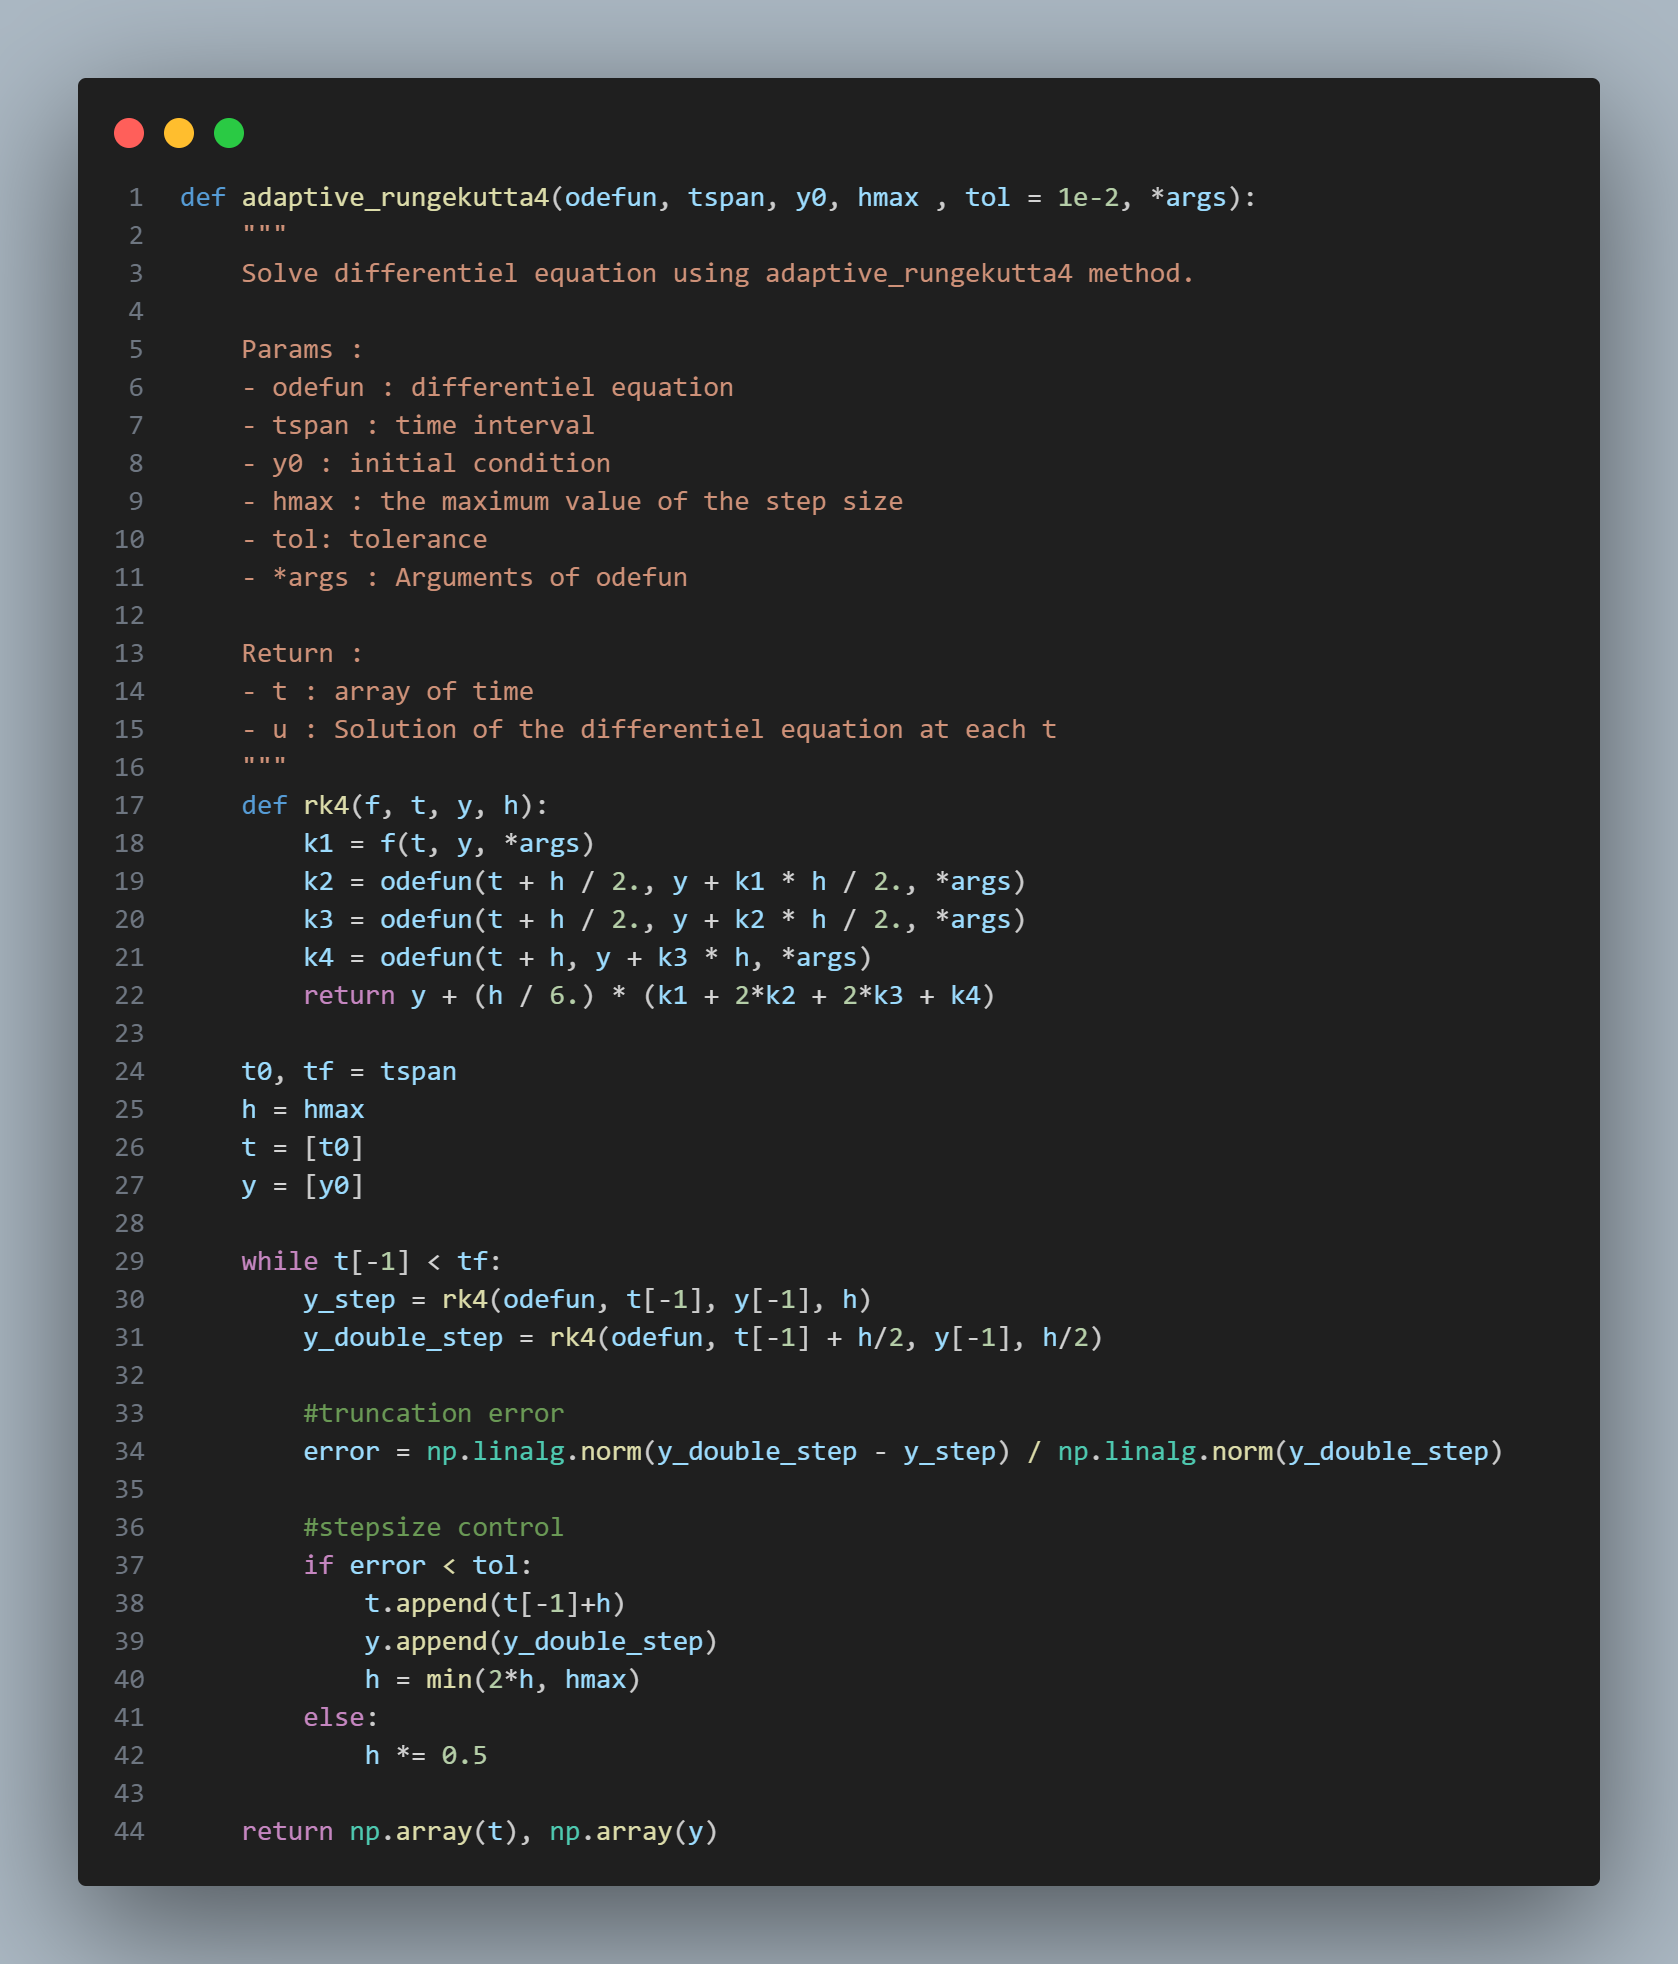
\includegraphics[width=0.78\textwidth]{img/adaptative_rk4.png}
%    \caption{Adaptive RK4}
%    \label{fig:4}
%\end{figure}




% --------------------------------------------------------------
%                            Conclusion
% --------------------------------------------------------------
\newpage
\section{Conclusion}
The application of the Ensemble Kalman Filter (EnKF) to the Lorenz system demonstrates its ability to track the chaotic dynamics of this nonlinear system despite the presence of noise and uncertainties. The results show that the EnKF can provide accurate estimates when filter parameters, such as the observation covariance matrix $R$ and the number of ensembles $N$, are carefully calibrated. An appropriate value of $R$ is crucial for balancing confidence between observations and model predictions, while a sufficient number of ensembles is essential for capturing the variability of the chaotic system. However, the filter has limitations, including high sensitivity to initialization errors and model parameters, which can affect the accuracy of estimates. To improve the filter's robustness and accuracy, future research should focus on optimizing ensemble initialization and developing methods to manage extreme uncertainties. In summary, the EnKF remains a powerful tool for managing complex dynamic systems, but continuous attention is needed to overcome its limitations and improve its performance under varying conditions.
\newpage
% --- Biblio par .bib
\bibliography{ref_Enkf.bib}
\vspace*{\fill}
%\selectlanguage{french}

%\begin{thebibliography}{7}
%\bibitem[Bastien 2019]{id-de-la-source}
%Auteurs : \emph{Un titre},  une date.
%\end{thebibliography}


\end{document}
